\chapter{Stradario della Parrocchia}
\label{chap:Stradario}

\begin{center}
\textbf{PARROCCHIA DI SAN FRANCESCO D’ASSISI}\\[0.5cm]
\textbf{STRADARIO 2011}
  %\scriptsize
	\small
	\begin{tabularx}{\textwidth}{| s | s | X |}
		\hline
		\multirow{2}{*}[-0pt]{\textbf{Nome via}} & 
		\textbf{inizio/fine dispari}&\textbf{numeri dispari}\\
		\cline{2-3}
		&\textbf{inizio/fine pari}&\textbf{numeri pari}\\
		\hline
		\multirow{2}{*}[-5pt]{via Berchet} &
		\multirow{2}{*}[-5pt]{tutta} &
		1, 3, 5, 7, 9, 11, 13, 15, 17, 19, 21, 23, 25, 27, 29, 31, 33, 35, 37\\
		\cline{3-3}
		&&2, 4, 6, 8, 10, 12, 12/1, 12/2, 14, 16, 18, 20, 22, 26\\
		\hline
		\multirow{2}{*}{via dei Bonomo} &
		\multirow{2}{*}{tutta} &
		1, 3, 5, 9, 11, 13, 15, 15/1, 17, 19\\
		\cline{3-3}
		&&2, 2/1, 2/2, 2/3, 2/4, 4\\
		\hline
		rotonda del Boschetto&
		tutta meno lato est &
		1, 2, 3, 3/1, 6\\
		\hline
		\multirow{2}{*}{androna Cesarotti} &
		\multirow{2}{*}{tutta} &
		1, 3, 5\\
		\cline{3-3}
		&&2, 4, 6, 8, 10\\
		\hline
		via di Cologna &
		lato dispari fra vie Kandler e Edera &
		25, 27, 27/1, 29, 29/1, 31, 33, 35, 37, 39, 41\\
		\hline
		\multirow{2}{*}{via dei Cunicoli} &
		\multirow{2}{*}{tutta} &
		1, 3, 5, 7, 9, 11, 13\\
		\cline{3-3}
		&&2, 4, 6, 8, 10\\
		\hline
		vicolo dell'Edera &
		dispari inizio via &
		1\\
		\hline
		\multirow{2}{*}{scala Ferolli} &
		\multirow{2}{*}{tutta} &
		1, 3\\
		\cline{3-3}
		&&4\\
		\hline
		\multirow{2}{*}{via Ferrari} & 
		lato dispari tutti&1, 3, 5, 7, 9, 11\\
		\cline{2-3}
		&lato pari inizio via&2\\
		\hline
		\multirow{2}{0.5\linewidth}[-30pt]{\centering via Giulia (finisce in rotonda del Boschetto)} &
		\multirow{2}{0.5\linewidth}[-30pt]{\centering da piazza Volontari Giuliani a fine} &
		41, 43, 45, 47, 49, 51, 53, 55, 57, 59, 61, 63, 65, 67, 69, 71, 73, 75, 75/1, 75/2, 75/3, 77, 79, 81, 83, 85\\
		\cline{3-3}
		&&24, 26, 28, 30, 32, 34, 36, 38, 48, 50, 52, 54, 54/1, 56, 58, 58/1, 60, 62, 64, 66, 68, 70, 72, 74, 76, 78, 80, 82, 84, 86, 88, 90,
		92, 94, 94/1, 96, 96/1, 98, 100, 102, 104, 108\\
		\hline
		\multirow{2}{0.5\linewidth}{\centering via Kandler (finisce in via Giulia) } &
		\multirow{2}{0.5\linewidth}{\centering da via di Cologna a fine} &
		7, 9, 11, 13, 15\bigstrut\\
		\cline{3-3}
		&&8, 10, 12, 14, 16\bigstrut\\
		\hline
		\multirow{2}{*}{via Margherita} &
		\multirow{2}{*}{tutta} &
		1, 5, 7, 9, 11, 13, 15, 19, 21, 23, 25\\
		\cline{3-3}
		&&2, 4, 4/1, 4/2, 4/3, 6, 8, 10\\
		\hline
		\multirow{2}{*}{via Mercantini} &
		\multirow{2}{*}{tutta} &
		1, 3, 5, 7, 9, 11, 11/1, 13\\
		\cline{3-3}
		&&2, 2/1, 4, 6, 8, 10, 12, 14\\
		\hline
		\multirow{2}{*}{scala al Monticello} &
		\multirow{2}{*}{tutta} &
		1, 3\\
		\cline{3-3}
		&&2, 4\\
		\hline
		\multirow{2}{*}{via dell’Oliveto} &
		\multirow{2}{*}{tutta} &
		1, 3, 5, 7, 9, 11\\
		\cline{3-3}
		&&2, 4\\
		\hline
		\multirow{2}{*}{via del Pilone} &
		\multirow{2}{*}{tutta} &
		1, 3, 5\\
		\cline{3-3}
		&&2, 4\\
		\hline
		\multirow{2}{*}[-5pt]{via Pindemonte} &
		\multirow{2}{*}[-5pt]{tutta} &
		1, 3, 5, 5/1, 7, 7/1, 7/2, 7/3, 9, 9/1, 9/2, 9/3, 9/4, 9/5, 11, 13\\
		\cline{3-3}
		&&2, 2/3, 4, 6, 8, 8/1, 8/2, 10, 10/1, 10/2, 12, 14\\
		\hline
		\multirow{2}{*}{via Pisoni} &
		\multirow{2}{*}{tutta} &
		1, 3, 5, 7, 9, 11, 13, 17\\*
		\cline{3-3}
		&&2, 4, 6, 10, 10/1, 12, 14, 18\\
		\hline
		vicolo dei Roveri&
		lato pari &
		2, 4, 6, 8, 10, 14, 16\\
		\hline
		\multirow{2}{*}[-5pt]{androna S. Cilino} &
		\multirow{2}{*}[-5pt]{tutta} &
		1, 3, 5, 7, 9, 11, 13, 15, 17, 19, 21, 23, 25\\
		\cline{3-3}
		&&2, 8, 10, 12, 14, 16, 18, 20, 22, 24, 26, 28, 30\\
		\hline
		\multirow{2}{*}{via S. Cilino} & 
		da inizio a v. S. Primo&1, 3, 5, 7, 9, 11, 13, 21, 23, 25, 27, 29\\
		\cline{2-3}
		&da inizio a v.Roveri&2, 4, 6\\
		\hline
		\multirow{2}{*}{via S. Donato} &
		\multirow{2}{*}{tutta} &
		1, 3, 5, 7, 9, 11, 13, 15, 21, 23\\
		\cline{3-3}
		&&2, 4, 6, 8, 10, 12, 14, 16, 20, 24, 26, 28\\
		\hline
		\multirow{2}{*}{via S. Felice} &
		\multirow{2}{*}{tutta} &
		1, 3, 5, 7\\
		\cline{3-3}
		&&2, 4, 6, 8, 10, 12, 14, 16\\
		\hline
		campo S. Luigi&
		lato v. Pindemonte &
		1, 1/1, 2, 3, 3/1, 4, 5, 6, 7\\
		\hline
		scala S. Luigi&
		lato pari&
		2\\
		\hline
		via S. Primo&
		dispari inizio via&
		1\\
		\hline
		\multirow{2}{0.5\linewidth}[-5pt]{\centering pendice dello Scoglietto} & 
		lato dispari tutti&1, 3, 3/1, 3/2, 5, 5/1, 5/2, 5/3, 5/4, 5/5, 5/6, 7, 7/1, 9, 11, 13, 13/1, 15, 17\\*
		\cline{2-3}
		&lato pari da inizio a vicolo dell’Edera&2, 4, 6, 8, 10, 12, 14, 16, 18\\
		\hline
		\multirow{2}{0.5\linewidth}{\centering via dello Scoglio (inizia in via Giulia)} &
		\multirow{2}{0.5\linewidth}{\centering da inizio a pendice Scoglietto} &
		1, 3, 5, 7, 9, 11, 13, 15, 17, 19, 21, 23, 25, 27, 29, 31, 33, 35, 37, 39, 51, 59, 61, 63, 67, 69, 71, 73, 75, 77, 83, 85, 87, 89, 
		91, 95, 97, 99, 103, 1077\\*
		\cline{3-3}
		&&2, 4, 6, 8, 12, 14, 14/1, 16, 18, 20\\
		\hline
		\multirow{2}{0.5\linewidth}[-5pt]{\centering viale XX Settembre (finisce in via Bonomo)} &
		\multirow{2}{0.5\linewidth}[-5pt]{\centering da piazza Volontari Giuliani a fine} &
		77, 79, 81, 83, 85, 87, 89, 89/1, 93, 97, 97/1, 101, 103\\*
		\cline{3-3}
		&&72, 74, 76, 78, 80, 82, 84, 86, 88, 90, 92, 94, 96, 98, 100, 100/1, 102, 102/1, 104\\
		\hline
		\multirow{2}{*}[-15pt]{via Verga} & 
		lato dispari tutti&1, 3, 9, 11, 13, 15, 17, 19\\
		\cline{2-3}
		&lato pari da inizio a via Zanella&2, 4, 6, 8, 8/1, 10, 12, 14, 16, 16/1, 18, 20, 20/2, 20/3, 22, 24, 26, 28, 30, 32, 34, 36, 38, 40,
		42, 42/1, 44, 44/1, 46, 48, 50, 52, 54, 56, 58\\
		\hline
		piazza Volontari Giuliani&
		tutta tolto lato ovest&
		1, 2, 3, 4, 5, 6, 7, 8\\
		\hline
		via Zanella&
		lato dispari da androna Cesarotti a fine (eccetto 129)&
		29, 31, 33, 35, 37, 41, 43, 45, 47, 49, 51, 53, 55, 57, 59, 61, 63, 65, 67, 69, 71, 73, 75, 77, 79, 81, 83, 85, 87, 89, 91, 95, 97, 99, 
		101, 103, 105, 107, 109, 111, 113, 115, 117, 119, 121, 123, 127\\
		\hline
	\end{tabularx}
\end{center}
\begin{center}
\needspace{3\baselineskip}
\textbf{NUMERI ANAGRAFICI}
  %\scriptsize
	\small
	\begin{tabularx}{\textwidth}{| s | X |}
		\hline
		località Chiadino&
		867\\
		\hline
		località Città&
		4922 (chiesa)\\
		\hline
	\end{tabularx}
\end{center}
\begin{center}
\textbf{VIE SENZA NUMERI}
  %\scriptsize
	\small
	\begin{tabularx}{\textwidth}{| s | X |}
		\hline
		piazzale Dreher&
		tra le vie Bonomo, Pindemonte, Giulia\\
		\hline
		bosco dei Pini&\\
		\hline
	\end{tabularx}
\end{center}
\begin{figure}[h]
\centering
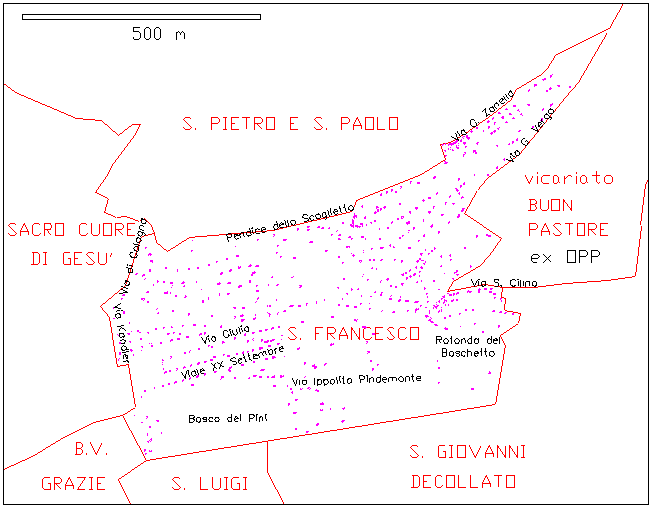
\includegraphics[
	width=0.8\textwidth
	]{immagini/mappa.png}%
\caption{Mappa della parrocchia di San Francesco.}
\end{figure}